Not all of the use cases listed in figure \ref{tab:actoreventtable} are sophisticated enough to be further described. Only the use cases \ucsproblem{} and solve problem are sophisticated enough to be described in detail. The rest are trivial enough to be omitted.
Another argument for omitting the rest is that the named use cases will be the most used in the system, the rest is merely for backend administration. 
The use case \ucsproblem{} is only used be the actor \aclient. Except for cases when \astaff{} or \sadmin{}  acts as \aclient{}. The use case is described in detail in figure \ref{fig:ucsproblem} and a use case diagram is showed in figure \ref{fig:submit_problem_use_case}. 


\begin{sadlist}[h]{\ucsproblem[c]}{Description of the use case submit problem.}{fig:ucsproblem}
\sadb{Use Case:} \ucsproblem[c] is initialized when a \aclient{} has a problem and wishes to submit that problem to the system in order to get help from the \astaff{}. 
He first has to select a category and from that choose one or more tags, he can change category and select even more tags. 
When the \aclient{} is done selecting tags the system compares the selected tags with other problems. 
If similar problems is found the \aclient{} is presented for the problems.
if one of these matches his particular problem, he can subscribe to the problem(if not closed), reopen problem(if closed), or use the information in the old problem to solve his problem independently. 
If no similar problem were found the \aclient{} creates a problem with a description and the previously selected tags. 
Hereafter the problem gets assigned to a \astaff{}. 

\sadb{Objects:} Problem, solution, tag, category, \client, \staff. (Department)

\sadb{Functions:} Search existing problems, compare problems, create problem, attach user to problem.


\end{sadlist}

\begin{figure}[htbp]
\begin{center}
 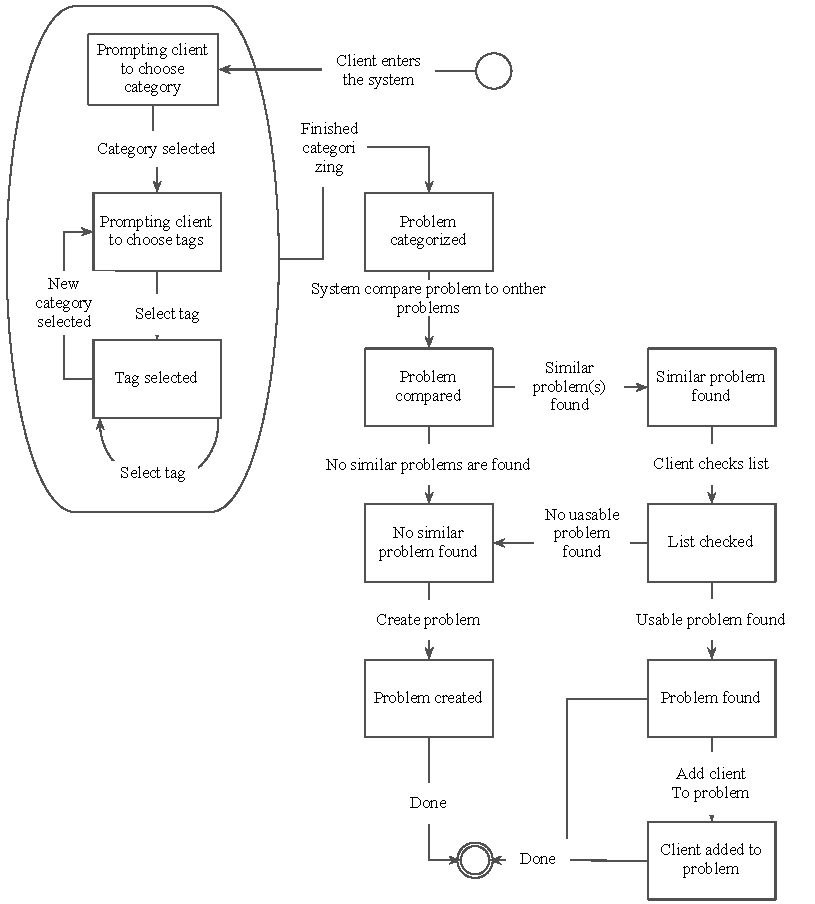
\includegraphics[scale=1]{input/application_domain_analysis/submit_problem_use_case}
\caption{A diagram of the use case \ucsproblem{}. The use case is described in detail in figure \ref{fig:ucsproblem}.}
\label{fig:submit_problem_use_case}
\end{center}
\end{figure}
